\chapter{Fully coalescent-based approaches to phylogeography}

Last time we saw an early example of using coalescent theory to
distinguish between two scenarios describing the history of
populations. In the example we considered, Knowles~\cite{Knowles-2001}
compared two scenarios, the ``widespread ancestor'' and the ``multiple
glacial refugia'' scenarios. To make the comparison she simulated data
under the ``widespread ancestor'' hypothesis, collected the samples
into a multiple-refuge tree, and calculated a statistic that measures
the discrepancy between the gene trees and the population trees. Her
observed gene tree was far less discordant than the simulated trees,
leading her to conclude that her grasshoppers had been dispersed among
multiple refugia in the past rather than being the remnants of a
single, widespread ancestral population. As I mentioned, one
limitation of the approach Knowles~\cite{Knowles-2001} takes is that
it requires the investigator to identify alternative scenarios before
beginning the analysis, and it can only identify which of the
scenarios is more likely than the others with which it is compared. It
cannot determine whether there are other scenarios that are even more
likely. Another approach is to back off a bit, specify a particular
process that we are interested in and to use what we know about that
process to try and estimate its properties.

\section*{Coalescent-based estimates of migration rate}

A few years before Knowles~\cite{Knowles-2001} appeared Beerli and
Felsenstein~\cite{Beerli-Felsenstein-1999,Beerli-Felsenstein-2001}
proposed a coalescent-based method to estimate migration rates among
populations. As with other analytical methods we've encountered in
this course, the details can get pretty hairy, but the basic idea is
(relatively) simple.\index{coalescent!migration}

Recall that in a single population we can describe the coalescent
history of a sample without too much difficulty. Specifically, given a
sample of $n$ alleles in a diploid population with effective size
$N_e$, the probability that the first coalescent event took place $t$
generations ago is
\begin{equation}
P(t|n, N_e) = \left(\frac{n(n-1)}{4N_e}\right)\left(1-
  \frac{n(n-1)}{4N_e}\right)^{t-1} \quad . \label{eq:coalescent-single}
\end{equation}
Now suppose that we have a sample of alleles from $K$ different
populations. To keep things (relatively) simple, we'll imagine that we
have a sample of $n$ alleles from every one of these populations and
that every population has an effective size of $N_e$. In addition,
we'll imagine that there is migration among populations, but again
we'll keep it really simple. Specifically, we'll assume that the
probability that a given allele in our sample from one population had
its ancestor in a different population in the immediately preceding
generation is $m$.\footnote{In other words, $m$ is the backwards
  migration rate, the probability that a gene in one population came
  from another population in the preceding generation. This is the
  same migration rate we encountered weeks ago when we discussed the
  balance between drift and migration.} Under this simple scenario, we
can again construct the coalescent history of our sample. How? Funny
you should ask.

We start by using the same logic we used to construct
equation~(\ref{eq:coalescent-single}). Specifically, we ask ``What's
the probability of an `event' in the immediately preceding
generation?'' The complication is that there are two kinds of events
possible: (1) a coalescent event and (2) a migration event. As in our
original development of the coalescent process, we'll assume that the
population sizes are large enough that the probability of two
coalescent events in a single time step is so small as to be
negligible. In addition, we'll assume that the number of populations
and the migration rates are small enough that the probability of more
than one event of either type is so small as to be negligible. That
means that all we have to do is to calculate the probability of either
a coalescent event or a migration event and combine them to calculate
the probability of an event. It turns out that it's easiest to
calculate the probability that there {\it isn't\/} an event first and
then to calculate the probability that there is an event as one minus
that.

We already know that the probability of a coalescent event in
population $k$, is
\[
P_k(\mbox{coalescent}|n, N_e) = \frac{n(n-1)}{4N_e} \quad ,
\]
so the probability that there is {\it not\/} a coalescent event in any
of our $K$ populations is
\[
P(\mbox{no coalescent}|n, N_e, K) = \left(1-\frac{n(n-1)}{4N_e}\right)^K
\quad .
\]
If $m$ is the probability that there was a migration event in a
particular population than the probability that there is {\it not\/} a
migration event involving any of our $nK$ alleles\footnote{$K$ populations
each with $n$ alleles} is
\[
P(\mbox{no migration}|m, K) = (1-m)^{nK} \quad .
\]
So the probability that there {\it is\/} an event of some kind is
\[
P(\mbox{event}|n, m, N_e, K) = 1 - P(\mbox{no coalescent}|n, N_e,
K)P(\mbox{no migration}|m, K) \quad .\label{eq:event}
\]
Now we can calculate the time back to the first event
\[
P(\mbox{event at }t|n, m, N_e, K) = P(\mbox{event}|n, m, N_e,
K)\left(1 - P(\mbox{event}|n, m, N_e, K)\right)^{t-1} \quad . \label{eq:time-to-event}
\]
We can then use Bayes theorem to calculate the probability that the
event was a coalescence or a migration and the populations
involved. Once we've done that, we have a new population configuration
and we can start over. We continue until all of the alleles have
coalesced into a single common ancestor, and then we have the complete
coalescent history of our sample.\footnote{This may not seem very
  simple, but just think about how complicated it would be if I
  allowed every population to have a different effective size and if I
  allowed each pair of populations to have different migration rates
  between them.} That's roughly the logic that Beerli and Felsenstein
use to construct coalescent histories for a sample of alleles from a
set of populations{\dash}except that they allow effective population
sizes to differ among populations and they allow migration rates to
differ among all pairs of populations. As if that weren't bad enough,
now things start to get even more complicated.

There are lots of different coalescent histories possible for a sample
consisting of $n$ alleles from each of $K$ different populations, even
when we fix $m$ and $N_e$. Worse yet, given any one coalescent
history, there are a lot of different possible mutational histories
possible. In short, there are a lot of different possible sample
configurations consistent with a given set of migration rates and
effective population size. Nonetheless, some combinations of $m$ and
$N_e$ will make the data more likely than others. In other words, we
can construct a likelihood for our data:
\[
P(\mbox{data}|m, N_e) \propto f(n, m, N_e, K) \quad ,
\]
where $f(n, m, N_e,K)$ is some very complicated function of the
probabilities we derived above. In fact, the function is so
complicated, we can't even write it down. Beerli and Felsenstein,
being very clever people, figured out a way to simulate the
likelihood, and {\tt Migrate} provides a (relatively) simple way that
you can use your data to estimate $m$ and $N_e$ for a set of
populations. In fact, {\tt Migrate} will allow you to estimate
pairwise migration rates among all populations in your sample, and
since it can simulate a likelihood, if you put priors on the
parameters you're interested in, i.e., $m$ and $N_e$, you can get
Bayesian estimates of those parameters rather than maximum likelihood
estimates, including credible intervals around those estimates so that
you have a good sense of how reliable your estimates are.\footnote{If
  you'd like to see a comparision of maximum likelihood and Bayesian
  approaches, Beerli~\cite{Beerli-2006} provides an excellent
  overview.}\index{coalescent!estimating migration rates}\index{migration!estimating}

There's one further complication I need to mention, and it involves a
lie I just told you. {\tt Migrate} can't give you estimates of $m$ and
$N_e$. Remember how every time we've dealt with drift and another
process we always end up with things like $4N_em$, $4N_e\mu$, and the
like. Well, the situation is no different here. What {\tt Migrate} can
actually estimate are the two parameters $4N_em$ and
$\theta=4N_e\mu$.\footnote{Depending on the option you pick when you
  run {\tt Migrate} you can either get $\theta$ and $4N_em$ or
  $\theta$ and $M=m/\mu$.} How did $\mu$ get in here when I only
mentioned it in passing? Well, remember that I said that once the
computer has constructed a coalescent history, it has to apply
mutations to that history. Without mutation, all of the alleles in our
sample would be identical to one another. Mutation is what what
produces the diversity. So what we get from {\tt Migrate} isn't the
fraction of a population that's composed of migrants. Rather, we get
an estimate of how much migration contributes to local population
diversity relative to mutation. That's a pretty interesting estimate
to have, but it may not be everything that we want.

There's a further complication to be aware of. Think about the
simulation process I described. All of the alleles in our sample are
descended from a single common ancestor. That means we are implicitly
assuming that the set of populations we're studying have been around
long enough and have been exchanging migrants with one another long
enough that we've reached a drift-mutation-migration equilibrium. If
we're dealing with a relatively small number of populations in a
geographically limited area, that may not be an unreasonable
assumption, but what if we're dealing with populations of crickets
spread across all of the northern Rocky Mountains? And what if we
haven't sampled all of the populations that
exist?\footnote{Beerli~\cite{Beerli-2004} discusses the impact of
  ``ghost'' populations. He concludes that you have to be careful
  about which populations you sample, but that you don't necessarily
  need to sample every population. Read the paper for the details.} In
many circumstances, it may be more appropriate to imagine that
populations diverged from one another at some time in the not too
distant past, have exchanged genes since their divergence, but haven't
had time to reach a drift-mutation-migration equilibrium. What do we
do then?

\section*{Divergence and migration}

Nielsen and Wakely~\cite{Nielsen-Wakeley-2001} consider the simplest
generalization of Beerli and
Felsenstein~\cite{Beerli-Felsenstein-1999,Beerli-Felsenstein-2001} you
could imagine~(Figure~\ref{fig:nielsen-wakeley}). They consider a
situation in which you have samples from only two populations and
you're interested in determining both how long ago the populations
diverged from one another and how much gene exchange there has been
between the populations since they diverged. As in {\tt Migrate}
mutation and migration rates are confounded with effective population
size, and the relevant parameters become:\index{coalescent!estimating migration}\index{coalescent!diverging populations}

\begin{itemize}

\item $\theta_a$, which is $4N_e\mu$ in the ancestral population.

\item $\theta_1$, which is $4N_e\mu$ in the first population.

\item $\theta_2$, which is $4N_e\mu$ in the second population.

\item $M_1$, which is $2N_em$ in the first population, where $m$ is
  the fraction of the first population composed of migrants from the
  second population.

\item $M_2$, which is $2N_em$ in the second population.

\item $T$, which is the time since the populations
  diverged. Specifically, if there have been $t$ units since
  the two populations diverged, $T=t/2N_1$, where $N_1$ is the
  effective size of the first population.

\end{itemize}

\begin{figure}
\begin{center}
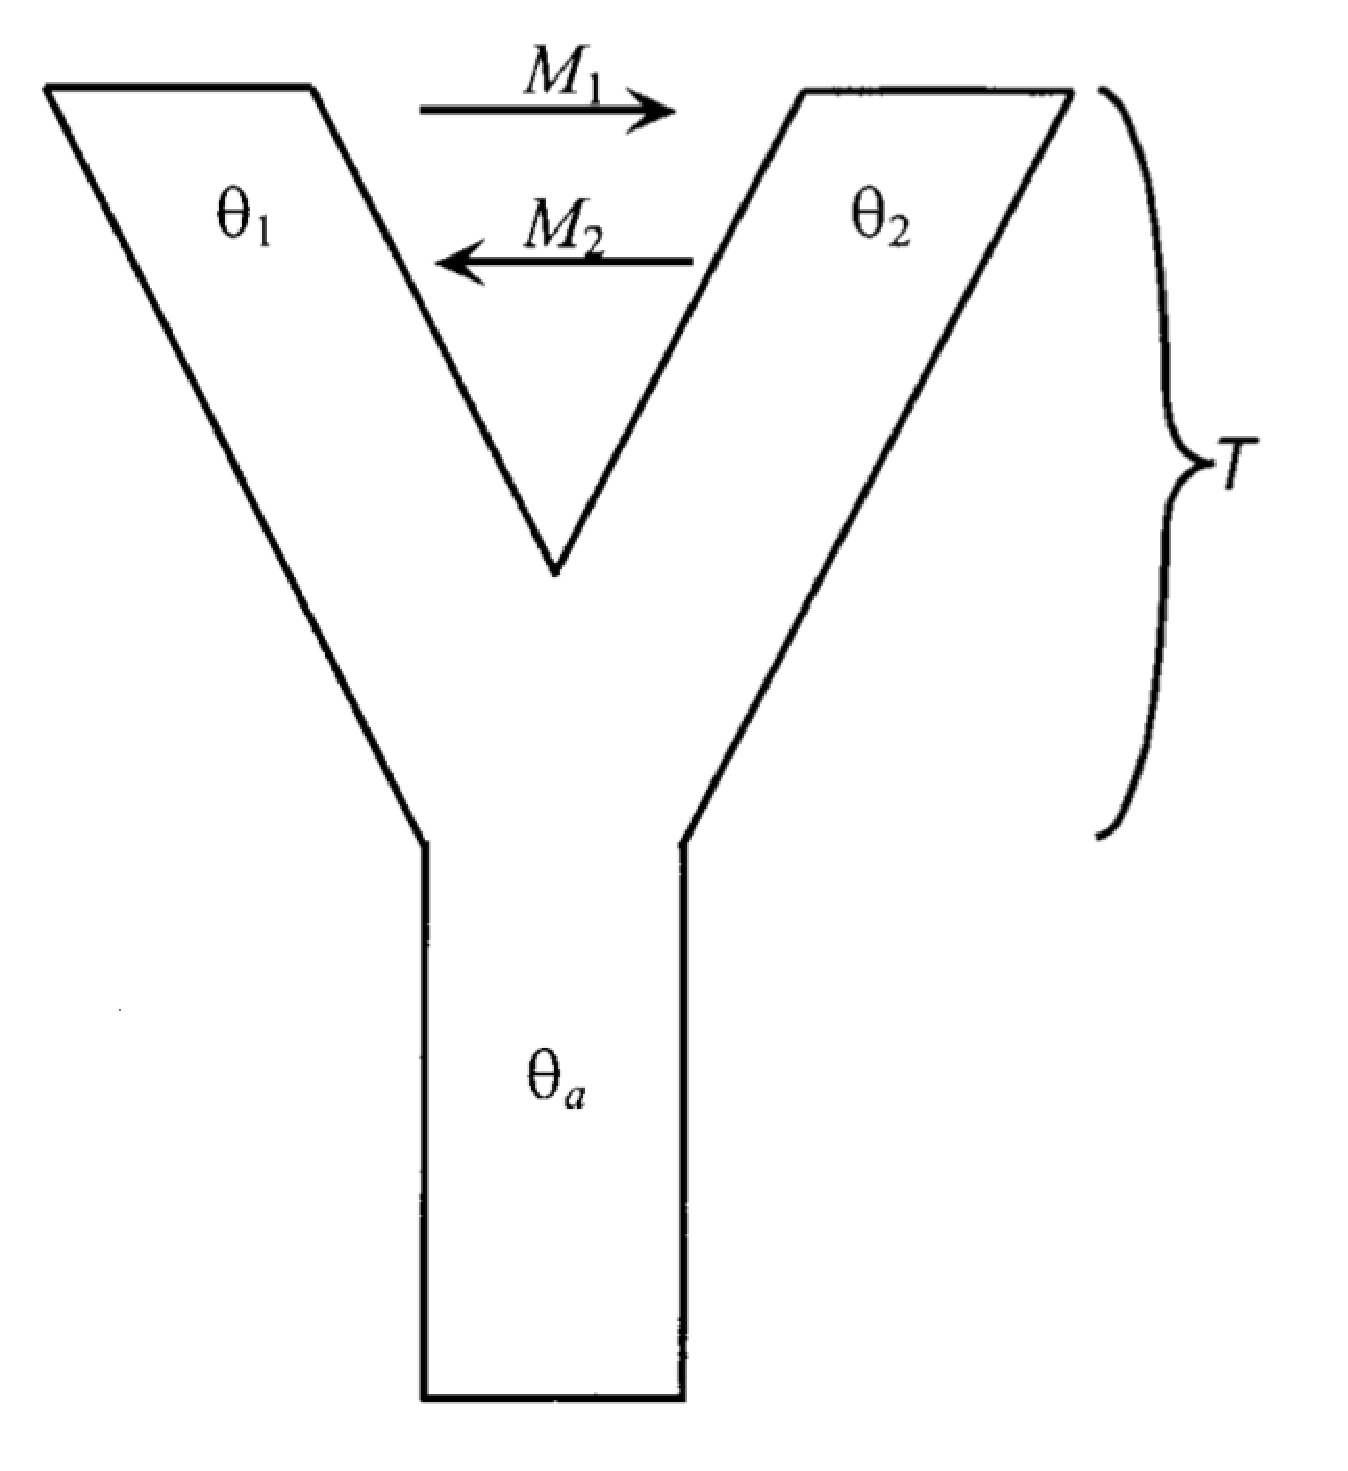
\includegraphics[height=6cm]{nielsen-wakeley.eps}
\end{center}
\caption{The simple model developed by Nielsen and
  Wakeley~\cite{Nielsen-Wakeley-2001}. $\theta_a$ is $4N_e\mu$ in the
  ancestral population; $\theta_1$ and $\theta_2$ are $4N_e\mu$ in the
  descendant populations; $M_1$ and $M_2$ are $2N_em$, where $m$ is
  the backward migration rate; and $T$ is the time since divergence of
  the two populations.}\label{fig:nielsen-wakeley}
\end{figure}

Given that set of parameters, you can probably imagine that you can
calculate the likelihood of the data for a given set of
parameters.\footnote{As with {\tt Migrate}, you can't calculate the
  likelihood explicitly, but you can approximate it
  numerically. See~\cite{Nielsen-Wakeley-2001} for details.} Once you
can do that you can either obtain maximum-likelihood estimates of the
parameters by maximizing the likelihood, or you can place prior
distributions on the parameters and obtain Bayesian estimates from the
posterior distribution. Either way, armed with estimates of
$\theta_a$, $\theta_1$, $\theta_2$, $M_1$, $M_2$, and $T$ you can say
something about: (1) the effective population sizes of the two
populations relative to one another and relative to the ancestral
population, (2) the relative frequency with which migrants enter each
of the two populations from the other, and (3) the time at which the
two populations diverged from one another. Keep in mind, though, that
the estimates of $M_1$ and $M_2$ confound local effective population
sizes with migration rates. So if $M_1 > M_2$, for example, it does
not mean that the fraction of migrants incorporated into population 1
exceeds the fraction incorporated into population 2. It means that the
impact of migration has been felt more strongly in population 1 than
in population 2.

\subsection*{An example}

Orti et al.~\cite{Orti-etal-1994} report the results of phylogenetic
analyses of mtDNA sequences from 25 populations of threespine
stickleback, {\it Gasterosteus aculeatus}, in Europe, North America,
and Japan. The data consist of sequences from a 747bp fragment of
cytochrome $b$. Nielsen and Wakely~\cite{Nielsen-Wakeley-2001} analyze
these data using their approach. Their analyses show that ``[a] model
of moderate migration and very long divergence times is more
compatible with the data than a model of short divergence times and
low migration rates.'' By ``very long divergence times'' they mean $T
> 4.5$, i.e., $t > 4.5N_1$. Focusing on populations in the western
(population 1) and eastern Pacific (population 2), they find that the
maximum likelihood estimate of $M_1$ is 0, indicating that there is
little if any gene flow from the eastern Pacific (population 2) into
the western Pacific (population 1). In contrast, the maximum
likelihood estiamte of $M_2$ is about 0.5, indicating that one
individual is incorporated into the eastern Pacific population from
the western Pacific population every other generation. The
maximum-likelihood estimates of $\theta_1$ and $\theta_2$ indicate
that the effective size of the population eastern Pacific population
is about 3.0 times greater than that of the western Pacific
population.

\subsection*{Extending the approach to multiple populations}

A couple of years ago, Jody Hey announced the release of {\tt
  IMa2}. Building on work described in Hey and
Nielsen~\cite{Hey-Nielsen-2004,Hey-Nielsen-2007}, {\tt IMa2} allows
you to estimate relative divergence times, relative effective
population sizes, and relative pairwise migration rates for more than
two populations at a time. That flexibility comes at a cost, of
course. In particular, you have to specify the phylogenetic history of
the populations before you begin the analysis.

